% !TEX TS-program = pdflatex
% !TEX encoding = UTF-8 Unicode
% !TEX root = ../ArsClassica.tex

%************************************************
\chapter{L'opera Sp.I.R.E}
\label{chp:L'opera Sp.I.R.E}
%************************************************

\epigraph{[...] bello come la retrattilità degli artigli degli uccelli rapaci; o ancora, come l'incertezza dei movimenti muscolari nelle pieghe delle parti molli della regione cervicale posteriore; [...] e soprattutto, come l'incontro fortuito su un tavolo di dissezione di una macchina da cucire e di un ombrello!}{Isidore Lucien Ducasse}

Tutto ebbe inizio nel luglio del 2017.

Nel corso della manifestazione \textit{ArteScienza} al Goethe Institute venne invitato il compositore francese, Pierre Jodlowski. Il suo lavoro compositivo \textit{Ombra della Mente} è ispirato ad alcuni scritti di Alda Merini durante le sue ricerche nei reparti psichiatrici.

Il lavoro di Jodlowski era basato su una parte teatrale recitata e una parte suonata da una clarinettista e cantata da una soprano (la stessa performer della voce recitante). La fusione tra momenti prettamente teatrali e parti musicali ebbero un effetto tagliente sulla mia produzione musicale successiva. Ogni intervento recitante era contrappuntato da rumori di strofinio di una matita su un foglio di carta e la frizione di una piccola molla presente nella meccanica della lampada di scena posizionata su uno scrittoio in palcoscenico. Tutto elaborato in live electronics. L'effetto della molla sfregata, amplificata da un microfono a contatto, mi ha fatto riaffiorare alla mente molti concerti di musica underground seguiti in passato (l'utilizzo delle molle, oltre ad appartenere all'universo della musica colta è stato abusato in ambienti musicali \textit{noise}\footnote{genere che utilizza il rumore come base principale per creare delle composizioni} e di musica cosiddetta "industriale" proprio per sottolineare l'utilizzo di materiale di scarto di industrie e fabbriche).

\begin{quotation}
Il paesaggio sonoro \textit{lo-fi} nasce dalla congestione sonora\footnote{R. Murray Schafer, \textit{Il paesaggio sonoro}, Casa Ricordi s.r.l. e LIM edizioni, 1985}.
\end{quotation}

Andando avanti negli studi ho notato, poi, che già negli anni 50 del Novecento, John Cage cercò, tramite l'utilizzo di elettromagneti e microfoni, di far percepire, amplificandoli, dei suoni non udibili. Dopo aver percorso durante il corso di \textit{interpretazione del partitura elettroacustica} assieme al Mº Giuseppe Silvi, tutto lo scenario cagiano, ho iniziato ad interessarmi in modo più serio all'universo delle molle e alle loro particolarità timbriche. Durante le mie ricerche è stato fortuito il lavoro fatto assieme al maestro Michelangelo Lupone al Centro di Ricerche Musicali (CRM) sito in Roma. \\
Aiutai il maestro alla creazione di una sua installazione nell'estate del 2017 assieme all'artista Licia Galizia: la scenografia interattiva della spettacolo coreutico \textit{Corpus 2.0}. L'utilizzo dei diffusori che montavamo all'interno delle opere installative e l'utilizzo di trasduttori piezoelettrici come parametri di controllo, mi ha fatto avvicinare ad un mondo a me limitrofo ma in parte sconosciuto.

\section{Necessità di uno strumento dedicato}
%\addcontentsline{toc}{section}{Necessità di uno strumento dedicato}

Durante le giornate di lavoro al CRM ogni materiale diventava fonte di ricerca sul suo utilizzo e sulle capacità timbriche. Ogni oggetto sonoro diventava frutto di studi sul timbro, anche minimi a volte per via dei tempi brevi dati dalle consegne, ma pieni di un universo sonoro al quale aggrapparsi. \\
Giorno per giorno si andava a materializzare un'idea sempre più nitida, fino al giorno del mio esame del III anno di composizione elettroacustica. \\
Un esercizio, un brano, un piccolo studio sulle armoniche del pianoforte, dove tutto partiva dalla trasformazione di un gesto sonoro, il pedale di risonanza in \textit{\textbf{fff}} e da una cellula sonora dalla quale poi, si formavano e alternavano momenti inarmonici con cluster e piccole volatine. Gesti e cellule sonore venivano elaborate tramite tre convoluzioni. Ogni convoluzione apparteneva ad un universo sonoro a sé:

\begin{itemize}
	\item{la prima convoluzione era la stessa cassa di risonanza del pianoforte eccitata dal pedale di risonanza calcato in \textit{\textbf{fff}};}
	\item{la seconda convoluzione era creata registrando la molla della stessa lampada da tavolo utilizzata da Pierre Jodlowski nel suo lavoro;}
	\item{la terza convoluzione era un'eccitazione del manico di una chitarra elettrica su un amplificatore a transistor.}
\end{itemize}

%\begin{floatingfigure}{10cm}
%\mbox{\epsfig{file=Prototipo0.jpg,width=9cm}}
%\small{\caption{\textit{particolare}}}
%\end{floatingfigure}

\begin{figure}[htbp]
\begin{center}
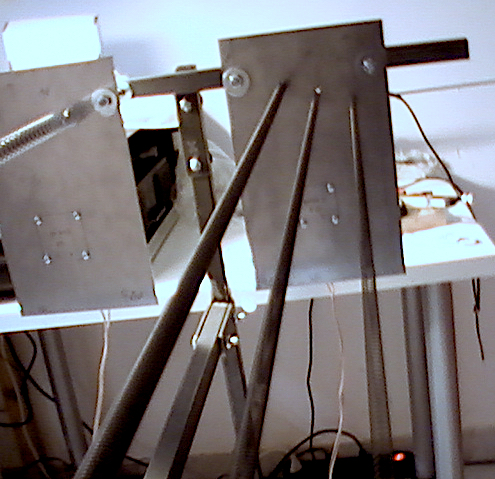
\includegraphics[]{../Graphics/Prototipo1.jpg}
\caption{particolare}
\label{default}
\end{center}
\end{figure}

Ogni convoluzione era quindi legata ad un gesto. Da qui alla creazione del mio iper-strumento, il passo è breve. Riuscii finalmente ad avere del tempo per finire di progettare il basamento, che prontamente un mio collega, Leonardo Mammozzetti ha provveduto a costruire, così da poter finalmente vedere e soprattutto sentire se tutte le mie idee portavano a qualcosa di reale. Era nato lo Sp.I.R.E. \\

\textit{Sp.I.R.E.}, acronimo di \textit{Springs Installation Regulated \& Enhanced}, fa riferimento alla fisicità del materiale che compone lo strumento. Ogni molla (\textit{spring}) è formata da \textit{spire}. Il numero di tali spire rende possibile, a seconda del materiale col quale vengono eccitate le molle, l'attivazione di armoniche e/o sub-armoniche.

%\begin{floatingfigure}{10cm}
%\mbox{\epsfig{file=Prototipo2.jpg,width=8cm}}
%\small{\caption{\textit{particolare}}}
%\end{floatingfigure}

\begin{figure}[htbp]
\begin{center}
\includegraphics[]{../Graphics/Prototipo2.jpg}
\caption{particolare}
\label{default}
\end{center}
\end{figure}

Userò quindi l'appellativo di Iper-strumento, perché è a tutti gli effetti uno strumento elettroacustico.

Questo esperimento è connesso allo studio di nuove identità formali relative alla natura dello strumento musicale.  La ricerca è unita ad una realtà installativa dell'opera, che induce chi guarda e ascolta, a toccare la materia e ad incuriosirsi verso materiali come molle e placche di metallo, che sono stati creati per scopi lontani dall'utilizzo che ne viene fatto in questo determinato caso.

Spiego sinteticamente. Un basamento unisce due placche di metallo che montano su di esse, 3 molle ciascuna, tese per la lunghezza paritaria di 80 centimetri.

Sp.i.r.e. è un progetto ambizioso che vuole, tra le altre cose, reinterpretare ed ampliare la visione di John Cage in Cartridge Music. Riuscire a rendere percepibili i suoni non udibili,  impercettibili, prodotti da una serie di molle a trazione, opportunamente amplificate, presenti sulla struttura.

Le molle sono disposte sul materiale a gradini, come se si andasse a suonare un violoncello, o un contrabbasso in posizione orizzontale. 
Ogni movimento sarà legato alle immagini di cordofoni classici, quindi durante la performance l'esecuzione avverrà con l'utilizzo di archetti per violoncello e contrabbasso. Da qui l'evoluzione del materiale in percussione o semplicemente in risonatore. 
L'installazione sarà interattiva: ogni tocco ricevuto dalle molle modificherà il segnale di sintesi che verrà propagato tramite gli attuatori, fissati sulla parete metallica.


\section{Intenzioni espressive}
\addcontentsline{toc}{section}{Intenzioni espressive (ideazione)}
\epigraph{\textbf{spirare} v. intr. e tr. [lat. spirare «soffiare»; respirare; emanare»]}
{\textit{Enciclopedia Treccani}}

L'intenzione espressiva era perciò, la creazione di uno strumento che avesse in sé sia un reverbero a molle che un reverbero a piastra. Il risultato fu esaltante: le molle sfregate con dita o archetti generavano un ambiente sonoro che le piastre amplificavano, dando vita a una sorta di convolutore naturale. So di estremizzare il senso di convoluzione, anche perché come sappiamo il convolutore è una sommatoria tra due segnali, uno legato ad un ambiente di ripresa e uno legato ad uno strumento suonante.

%\begin{floatingfigure}{10cm}
%\mbox{\epsfig{file=Prototipo3.jpg,width=9cm}}
%\small{\caption{\textit{particolare}}}
%\end{floatingfigure}

\begin{figure}[htbp]
\begin{center}
\includegraphics[]{../Graphics/Prototipo3.jpg}
\caption{particolare}
\label{default}
\end{center}
\end{figure}

La svolta decisiva la ebbi durante il montaggio di Sp.I.R.E. perché decisi di aggiungere una variante elettroacustica: aggiunsi degli attuatori. Gli attuatori, diffusori a parete capaci di far interagire il materiale sul quale sono collocati con il suono diffuso, erano la variante finale per la messa a punto finale dell'opera.
Come scrive Silvia Lanzalone:
\begin{quotation}
La catena elettroacustica, nonostante il notevole perfezionamento tecnologico degli ultimi decenni verso l'accuratezza della riproduzione sonora, conferisce ancora al suono una trasformazione finale dovuta alla natura elettromeccanica dei suoi componenti, imponendovi dunque una deformazione che la rende decorrelata dal segnale che trasmette, nonché estranea ad esso dal punto di vista della sua identificazione percettiva nello spazio destinato alla sua diffusione\footnote{Silvia Lanzalone \textit{Strumenti aumentati} in \footnote{Acustica} UTET}.
\end{quotation} 

Spesso, quasi sempre, il suono elettronico risulta 

Per messa a punto finale intendo ovviamente la creazione di un ambiente di lavoro da quale partire per poter sia iniziare i primi studi sul timbri, ma soprattutto, per iniziare a scrivere una composizione scritta ad hoc per Sp.I.R.E.. \\

\section{Intenzioni estetiche}
\addcontentsline{toc}{section}{Intenzioni estetiche}
Il progetto va a rappresentare il legame con ciò che abbiamo attorno a noi, quello che siamo: tutt'uno con la metropoli e con l'ambiente che la circonda e va a formarla.

Questa è l'identità di Sp.i.r.e., finalmente si tocca con mano la parte nascosta della materia, il lato più nascosto di quello che vediamo attorno a noi. In unione ai suoni non udibili e all'invisibile, si scorge un richiamo verso una visione immaginifica che porta fino a dentro la nostra anatomia. Come se le spire della molla potessero essere ricondotte ai ripiegamenti dell'intestino; come se, all'eccitazione di una molla, si riconducesse la possibilità di produrre delle sub-armoniche e in qualche modo, di avvicinarsi alle vibrazioni interne dell'anatomia umana.

La meccanica, l'elettronica e i suoni analogici, rendono possibile la creazione di un mondo nuovo, e l'eccitazione delle molle mediante le placche di metallo fa sì che questa dimensione diventi parte della realtà umana. \\
Vengono a formarsi più dimensioni d'ascolto e più dimensioni tattili, causate dalle diverse eccitazioni del materiale. A queste dimensioni d'ascolto si unisce la diffusione audio della performance, che sarà omnidirezionale e renderà possibile coprire tutto il panorama d'ascolto.

Così Sp.i.r.e., anche nella sua identità installativa, respira ed emana il segnale elettroacustico in almeno due dimensioni d'ascolto:

\begin{enumerate} 
\item{\textit{Analogica}, la risposta del materiale ai suoni sintetici e al tocco umano}
\item{\textit{Elettrica ed elettronica}, che prende vita grazie ai suoni di sintesi diffusi dagli attuatori}
\end{enumerate}

